\chapter{Mesures d'admittances sur instruments à cordes pincées}
Dans cette partie nous procédons à la mesure d'admittance (accélération sur force) d'une guitare et d'un Ukulélé au niveau du point de couplage entre la corde et le corps.
\section{Nomenclature des grandeurs physiques :} 
\begin{itemize}
\item $Y_{body,indices}$ : Admittance du corps. l'indice $1$ indique l'axe vertical et l'indice $2$ l'axe horizontal.
\item $Y_{string,indices}$ : Admittance de la corde.
\item $Y_{total,string,indices}$ : Admittance de l'ensemble corde+corps.
\item $y_{string,wire}$ : signal temporel de la corde excitée au fil.
\item $F$ : Force appliquée par le marteau 
\item $\alpha$ : Accélération délivrée par le capteur 
\end{itemize}

\section{Dispositif de mesure employé}
Pour nos mesures, nous disposons de :
\begin{itemize}
\item un capteur tri-axes
\item un marteau d'impulsion
\item une carte d'acquisition NI
\item un amplificateur
\item un système d'acquisition sur matlab
\item un microphone
\item une guitare
\end{itemize}
En amont de nos mesures, nous renseignons la fréquence d'échantillonnage et la sensibilité du capteur dans le code d'acquisition. Le marteau d'impulsion fourni la force d'impacte $F$ sur la guitare. 

Lors de l'acquisition de nos résultats, le signal d'impulsion du marteau est fenétré dans le temps autour de son attaque dans le but d'eliminer le bruit électronique, dont on veut ignorer l'influence . 

Au final nous récupérons, la réponse temporelle de l'accélération en 2D et de la force. On obtient également leur réponse fréquentielle, c'est le rapport des deux, qui donne l'admittance du système.

L'installation du banc de mesure est présenté en Annexe. %dans la Figure \ref{fig:gull}.

%\begin{figure}[h]
%centering
%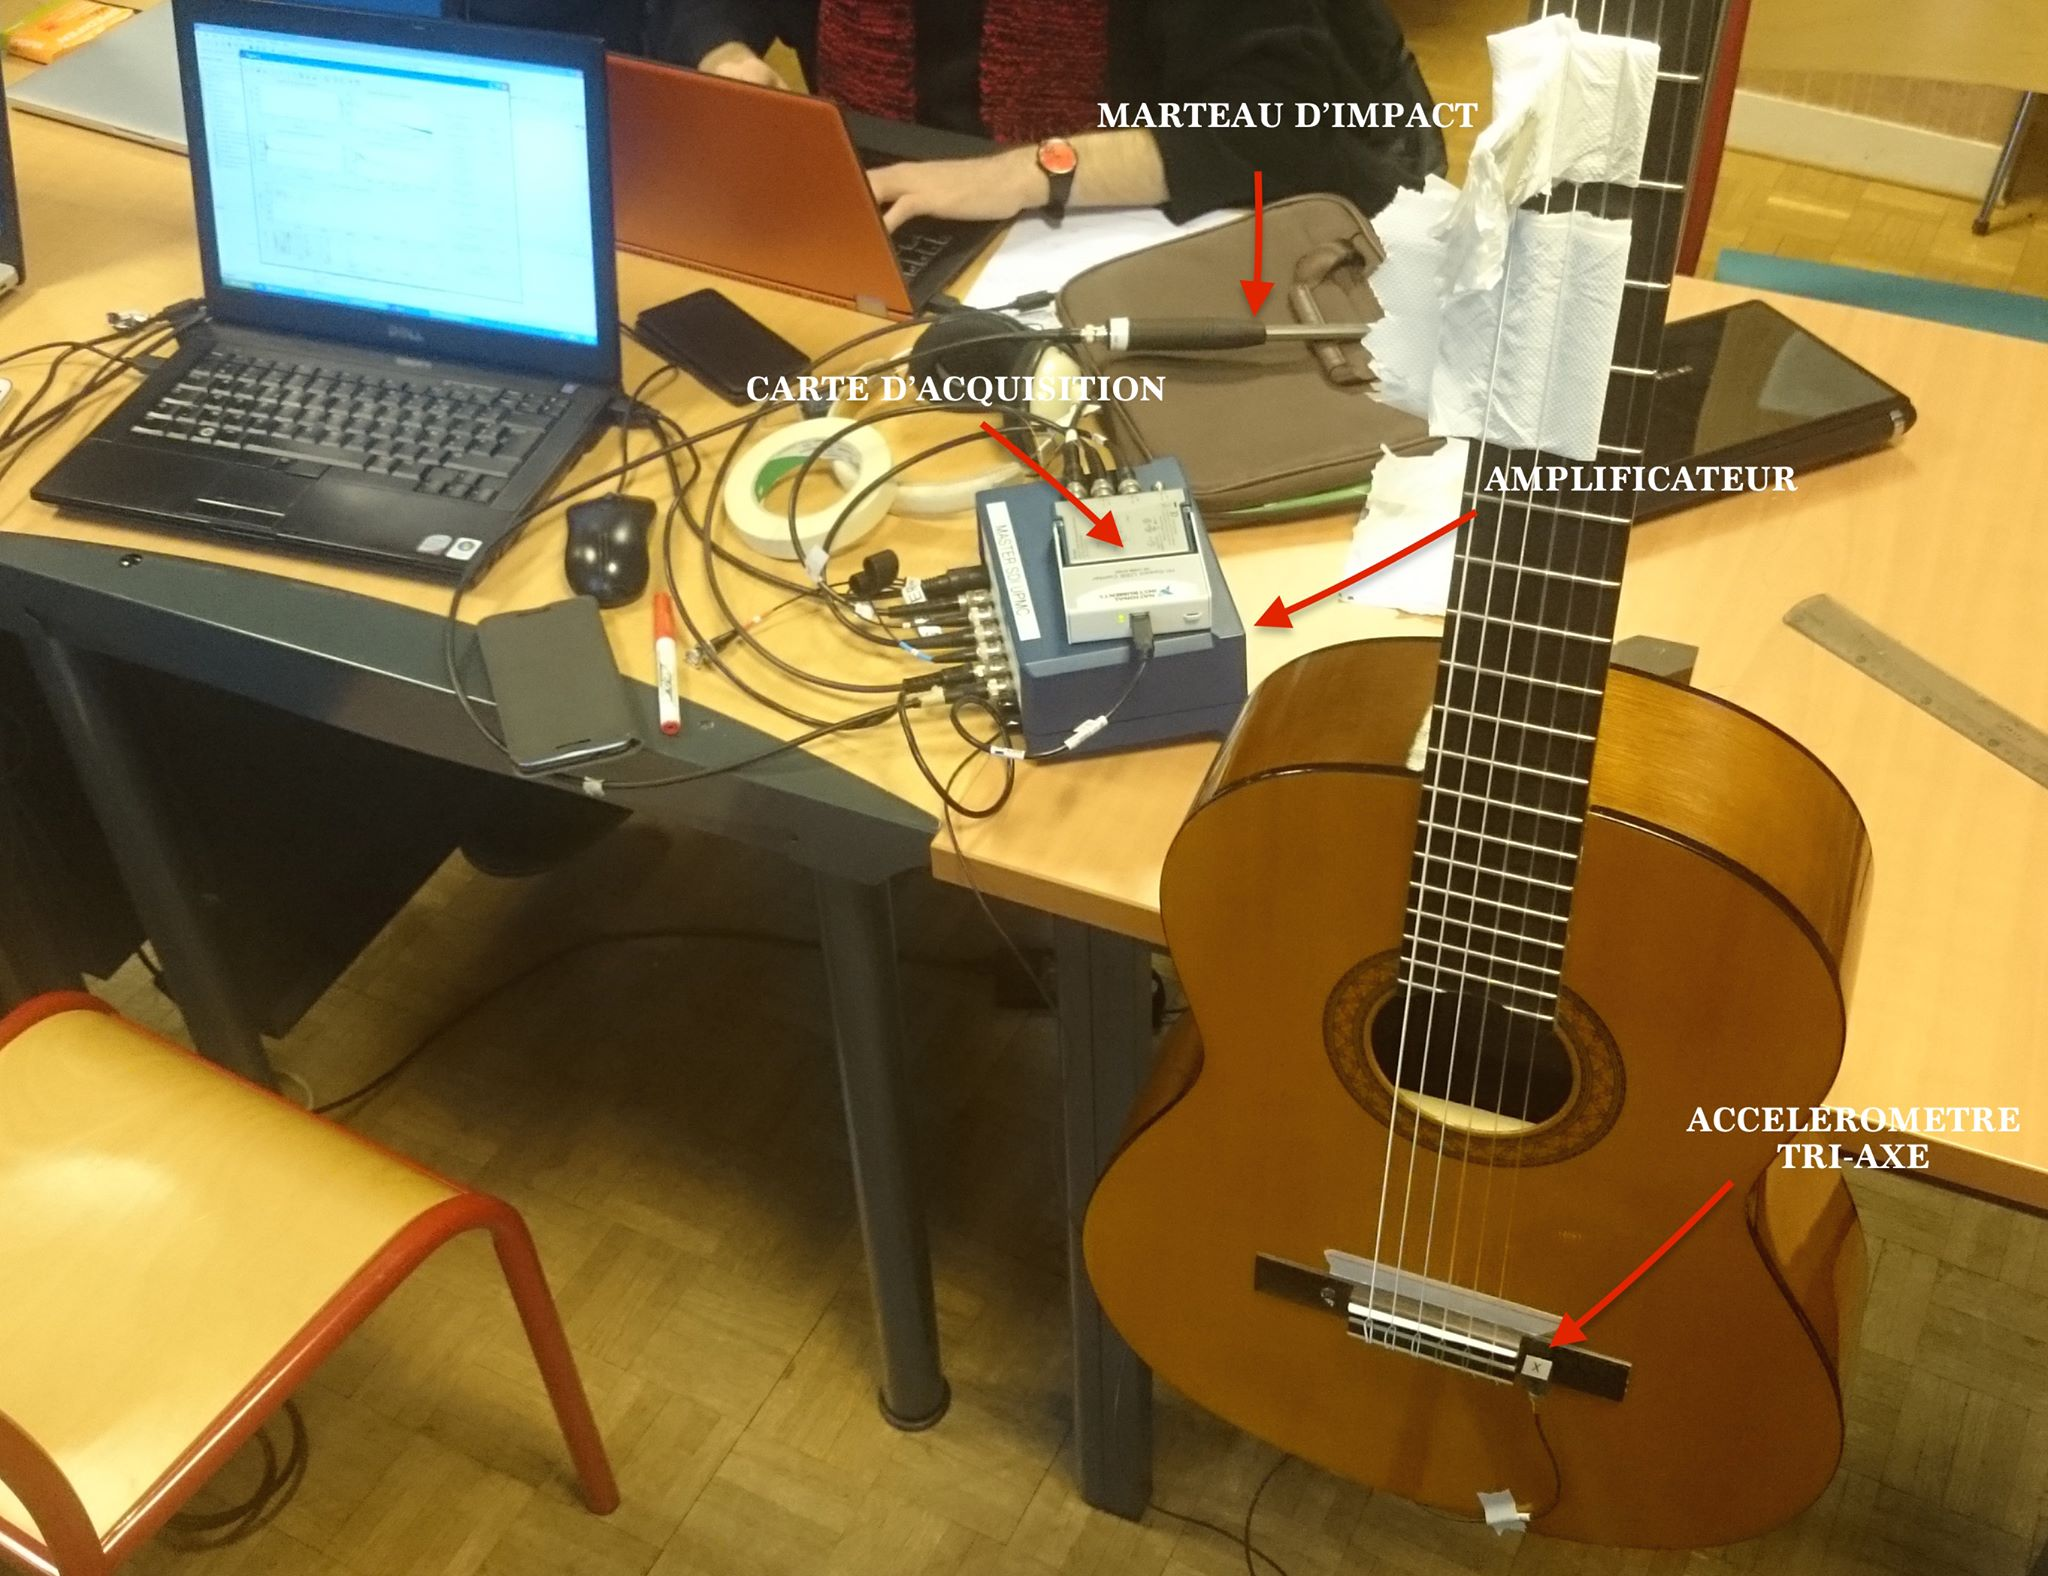
\includegraphics[width = 7cm]{dispo.JPG}
%\caption{Dispositif de mesure}
%\label{fig:gull}
%\end{figure}

\section{Protocole de mesures}
Voici l'ensemble des mesures effectuées. Pour assurer une répétablité de la mesure, elles seront faites 5 fois chacune dans le même temps. Nous choisissons une valeur de fréquence d'echantillonnage pour l'accéléromètre de  $F_e = 25600Hz$.
\begin{itemize}
\item Le corps seul, axe vertical(les cordes sont étouffées).
\item Le corps et la corde de Mi2, axe vertical et horizontal.
\item Le corps et la corde de Mi4, axe vertical et horizontal.
\item La corde Mi4 excitée au fil perpendiculairement à la table.
\item La corde Mi4 excitée au fil à $45$ degré de la table.
\item Mesure du rayonnement de la table seule.
\end{itemize}
Les deux dernières mesures consistent en l'excitation de la corde avec un fil de cuivre à une distance b = 17 mm du chevalet. 

\section{Commentaire et exploitation des résultats}
\subsection{Visualisation des résultats}
La Figure \ref{fig:goll} montre l'ensemble de nos résultats d'admittance pour le corps seul, mesuré au niveau de la corde de Mi4 : 
\begin{figure}[h]
\centering
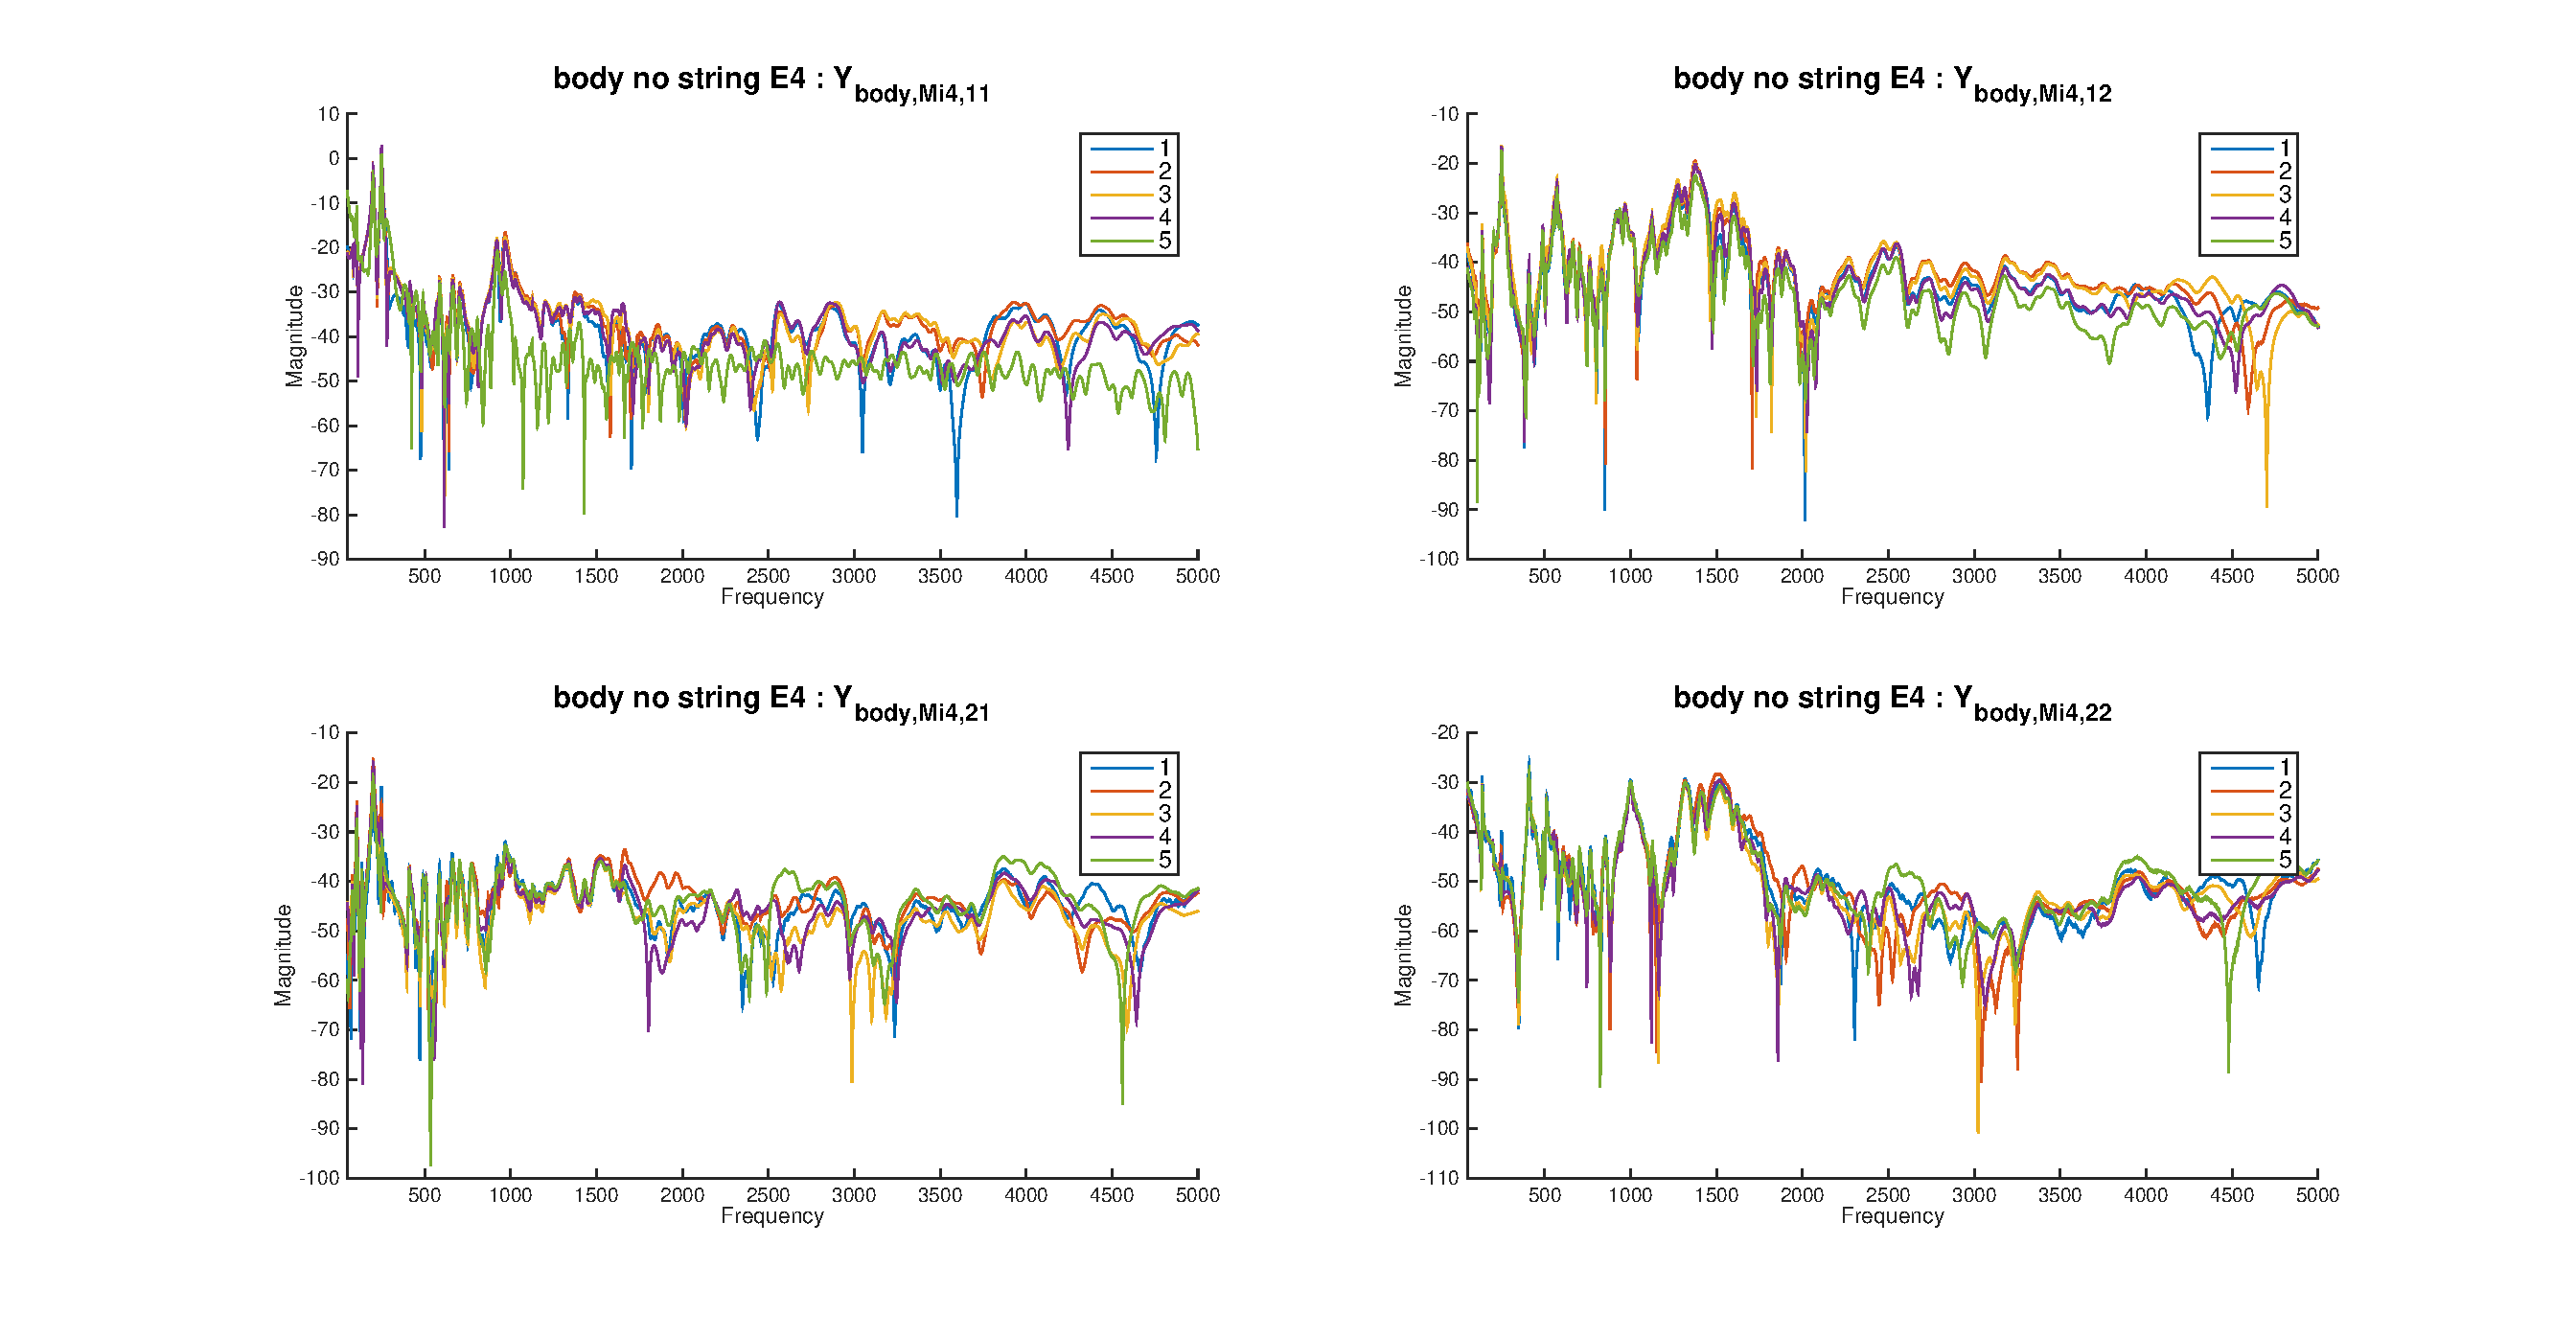
\includegraphics[width = 14cm]{figures/Y_body_E4.eps}
\caption{Mesures pour le corps au niveau du chevalet et de la corde de Mi4}
\label{fig:goll}
\end{figure}
La première ligne correspond à la mesure avec impulsion normale à la table, la seconde ligne, à une impulsion parallèle. On obtient deux dimensions de l'admittance pour ces mesures, effectuées 5 fois chacune. Pour nos synthèses, nous ne nous servirons que de l'admittance correspondant au déplacement transversal de la table ($Y_{body,11}$, $Y_{body,12}$ et $Y_{body,21}$) doivent être semblable.

\subsection{Calcul de la cohérence}
Dans le but de juger de la viabilité de nos mesures, nous calculons la cohérence des 5 mesures de $Y_{body,11}$ au niveau de la corde de Mi2 et de la corde de Mi4. La Figure \ref{fig:goll},  montre dans le graphe de $Y_{body,11}$ une mesure (la 5ème) que nous pourrons ignorer dans ce calcul. Les chutes locales de cohérence observées avant 2000Hz sont généralement dues à des anti-résonances autour desquelles les valeurs très faibles mesurées peuvent être assimilées à un bruit statistique.


\begin{figure}[h]
\centering
\begin{tabular}{cc}
   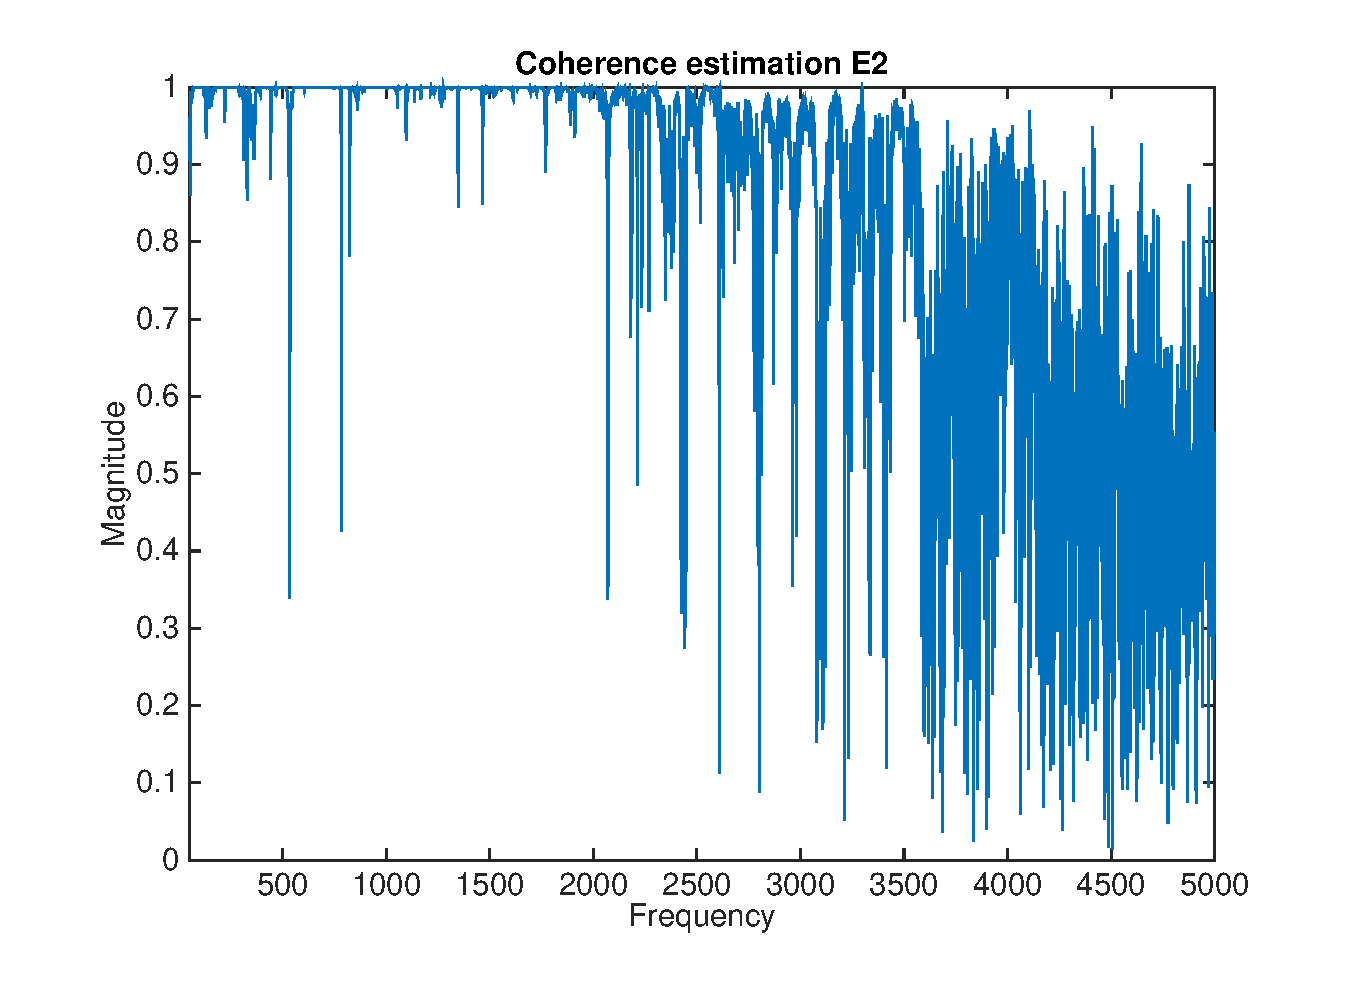
\includegraphics[width = 5cm]{figures/coherence_Z_1_E2.eps} &
   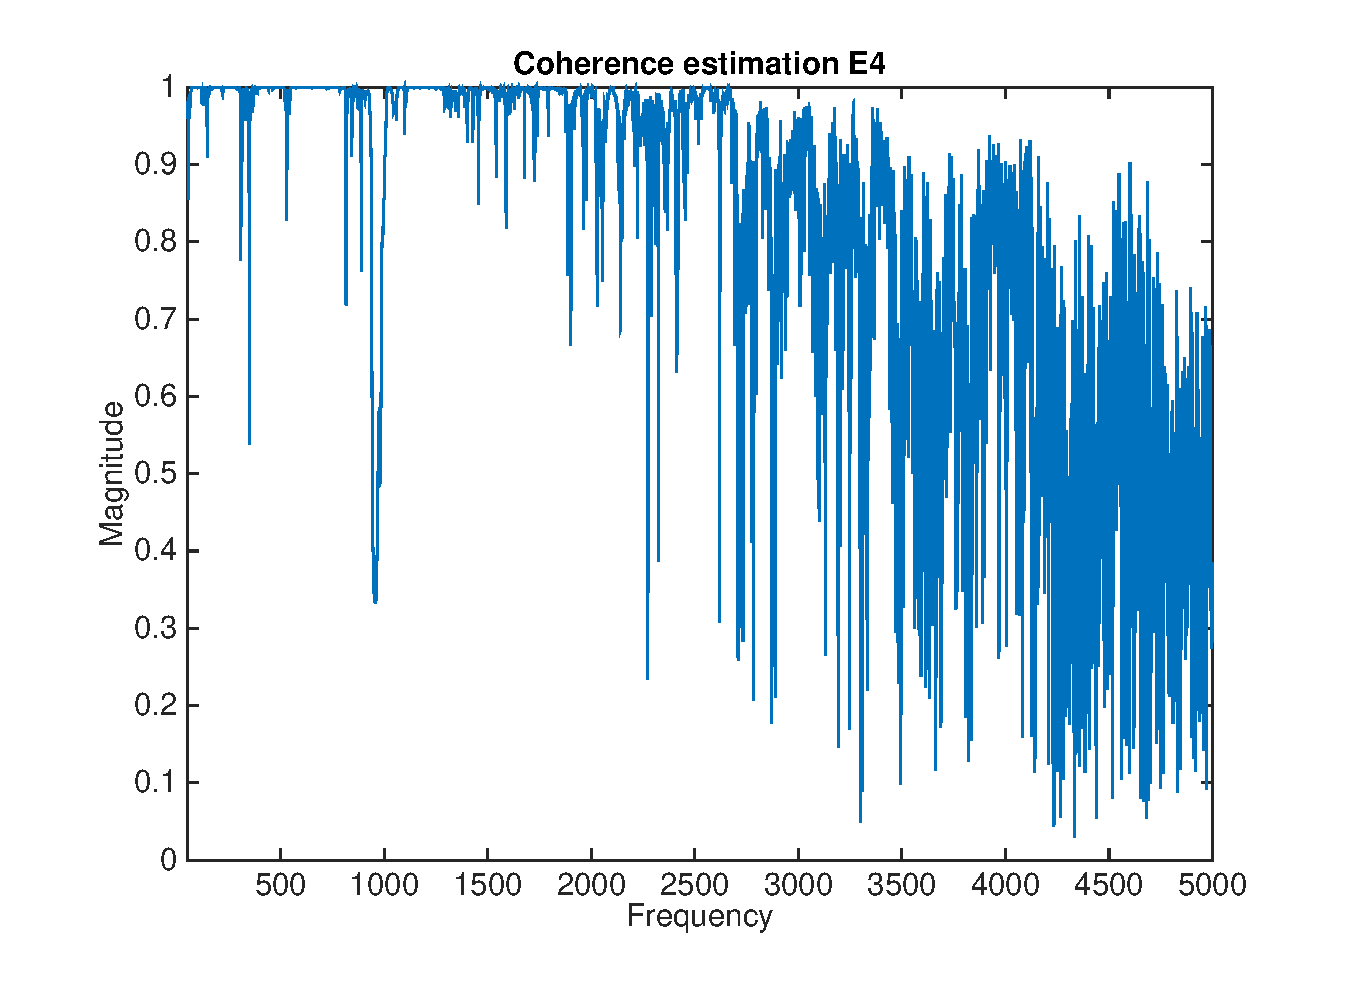
\includegraphics[width = 5cm]{figures/coherence_Z_1_E4.eps} \\
\end{tabular}
\caption{Cohérence des mesures Ybody1 au niveau de la corde de Mi2 et de celle de Mi4}
\label{fig:gall}
\end{figure}
Nous observons sur la Figure \ref{fig:gall} une baisse importante de la cohérence autour de la fréquence de 2000 Hz. Cela est dû à un filtrage passe-bas du marteau qui ne produit pas une impulsion parfaitement ponctuelle lors de l'excitation. Nous pourrons donc dans nos synthèse, limiter notre recherche des modes de corps à la région fréquentielle entre 0 et 2000 Hz.
